% 2-15-rb-tree.tex

%%%%%%%%%%%%%%%%%%%%
\documentclass[a4paper, justified]{tufte-handout}

% hw-preamble.tex

% geometry for A4 paper
% See https://tex.stackexchange.com/a/119912/23098
\geometry{
  left=20.0mm,
  top=20.0mm,
  bottom=20.0mm,
  textwidth=130mm, % main text block
  marginparsep=5.0mm, % gutter between main text block and margin notes
  marginparwidth=50.0mm % width of margin notes
}

% for colors
\usepackage{xcolor} % usage: \color{red}{text}
% predefined colors
\newcommand{\red}[1]{\textcolor{red}{#1}} % usage: \red{text}
\newcommand{\blue}[1]{\textcolor{blue}{#1}}
\newcommand{\teal}[1]{\textcolor{teal}{#1}}

\usepackage{todonotes}

% heading
\usepackage{sectsty}
\setcounter{secnumdepth}{2}
\allsectionsfont{\centering\huge\rmfamily}

% for Chinese
\usepackage{xeCJK}
\usepackage{zhnumber}
\setCJKmainfont[BoldFont=FandolSong-Bold.otf]{FandolSong-Regular.otf}

% for fonts
\usepackage{fontspec}
\newcommand{\song}{\CJKfamily{song}} 
\newcommand{\kai}{\CJKfamily{kai}} 

% To fix the ``MakeTextLowerCase'' bug:
% See https://github.com/Tufte-LaTeX/tufte-latex/issues/64#issuecomment-78572017
% Set up the spacing using fontspec features
\renewcommand\allcapsspacing[1]{{\addfontfeature{LetterSpace=15}#1}}
\renewcommand\smallcapsspacing[1]{{\addfontfeature{LetterSpace=10}#1}}

% for url
\usepackage{hyperref}
\hypersetup{colorlinks = true, 
  linkcolor = teal,
  urlcolor  = teal,
  citecolor = blue,
  anchorcolor = blue}

\newcommand{\me}[4]{
    \author{
      {\bfseries 姓名:}\underline{#1}\hspace{2em}
      {\bfseries 学号:}\underline{#2}\hspace{2em}\\[10pt]
      {\bfseries 评分:}\underline{#3\hspace{3em}}\hspace{2em}
      {\bfseries 评阅:}\underline{#4\hspace{3em}}
  }
}

% Please ALWAYS Keep This.
\newcommand{\noplagiarism}{
  \begin{center}
    \fbox{\begin{tabular}{@{}c@{}}
      请独立完成作业,不得抄袭。\\
      若得到他人帮助, 请致谢。\\
      若参考了其它资料,请给出引用。\\
      鼓励讨论,但需独立书写解题过程。
    \end{tabular}}
  \end{center}
}

\newcommand{\goal}[1]{
  \begin{center}{\fcolorbox{blue}{yellow!60}{\parbox{0.50\textwidth}{\large 
    \begin{itemize}
      \item 体会``思维的乐趣''
      \item 初步了解递归与数学归纳法 
      \item 初步接触算法概念与问题下界概念
    \end{itemize}}}}
  \end{center}
}

% Each hw consists of four parts:
\newcommand{\beginrequired}{\hspace{5em}\section{作业 (必做部分)}}
\newcommand{\beginoptional}{\section{作业 (选做部分)}}
\newcommand{\beginot}{\section{Open Topics}}
\newcommand{\begincorrection}{\section{订正}}
\newcommand{\beginfb}{\section{反馈}}

% for math
\usepackage{amsmath, mathtools, amsfonts, amssymb}
\newcommand{\set}[1]{\{#1\}}

% define theorem-like environments
\usepackage[amsmath, thmmarks]{ntheorem}

\theoremstyle{break}
\theorempreskip{2.0\topsep}
\theorembodyfont{\song}
\theoremseparator{}
\newtheorem{problem}{题目}[subsection]
\renewcommand{\theproblem}{\arabic{problem}}
\newtheorem{ot}{Open Topics}

\theorempreskip{3.0\topsep}
\theoremheaderfont{\kai\bfseries}
\theoremseparator{:}
\theorempostwork{\bigskip\hrule}
\newtheorem*{solution}{解答}
\theorempostwork{\bigskip\hrule}
\newtheorem*{revision}{订正}

\theoremstyle{plain}
\newtheorem*{cause}{错因分析}
\newtheorem*{remark}{注}

\theoremstyle{break}
\theorempostwork{\bigskip\hrule}
\theoremsymbol{\ensuremath{\Box}}
\newtheorem*{proof}{证明}

% \newcommand{\ot}{\blue{\bf [OT]}}

% for figs
\renewcommand\figurename{图}
\renewcommand\tablename{表}

% for fig without caption: #1: width/size; #2: fig file
\newcommand{\fig}[2]{
  \begin{figure}[htbp]
    \centering
    \includegraphics[#1]{#2}
  \end{figure}
}
% for fig with caption: #1: width/size; #2: fig file; #3: caption
\newcommand{\figcap}[3]{
  \begin{figure}[htbp]
    \centering
    \includegraphics[#1]{#2}
    \caption{#3}
  \end{figure}
}
% for fig with both caption and label: #1: width/size; #2: fig file; #3: caption; #4: label
\newcommand{\figcaplbl}[4]{
  \begin{figure}[htbp]
    \centering
    \includegraphics[#1]{#2}
    \caption{#3}
    \label{#4}
  \end{figure}
}
% for margin fig without caption: #1: width/size; #2: fig file
\newcommand{\mfig}[2]{
  \begin{marginfigure}
    \centering
    \includegraphics[#1]{#2}
  \end{marginfigure}
}
% for margin fig with caption: #1: width/size; #2: fig file; #3: caption
\newcommand{\mfigcap}[3]{
  \begin{marginfigure}
    \centering
    \includegraphics[#1]{#2}
    \caption{#3}
  \end{marginfigure}
}

\usepackage{fancyvrb}

% for algorithms
\usepackage[]{algorithm}
\usepackage[]{algpseudocode} % noend
% See [Adjust the indentation whithin the algorithmicx-package when a line is broken](https://tex.stackexchange.com/a/68540/23098)
\newcommand{\algparbox}[1]{\parbox[t]{\dimexpr\linewidth-\algorithmicindent}{#1\strut}}
\newcommand{\hStatex}[0]{\vspace{5pt}}
\makeatletter
\newlength{\trianglerightwidth}
\settowidth{\trianglerightwidth}{$\triangleright$~}
\algnewcommand{\LineComment}[1]{\Statex \hskip\ALG@thistlm \(\triangleright\) #1}
\algnewcommand{\LineCommentCont}[1]{\Statex \hskip\ALG@thistlm%
  \parbox[t]{\dimexpr\linewidth-\ALG@thistlm}{\hangindent=\trianglerightwidth \hangafter=1 \strut$\triangleright$ #1\strut}}
\makeatother

% for footnote/marginnote
% see https://tex.stackexchange.com/a/133265/23098
\usepackage{tikz}
\newcommand{\circled}[1]{%
  \tikz[baseline=(char.base)]
  \node [draw, circle, inner sep = 0.5pt, font = \tiny, minimum size = 8pt] (char) {#1};
}
\renewcommand\thefootnote{\protect\circled{\arabic{footnote}}} % feel free to modify this file
%%%%%%%%%%%%%%%%%%%%
\title{第3-4讲: 用于动态等价关系的数据结构}
\me{林凡琪}{211240042}{}{}
\date{\zhtoday} % or like 2019年9月13日
%%%%%%%%%%%%%%%%%%%%
\begin{document}
\maketitle
%%%%%%%%%%%%%%%%%%%%
\noplagiarism % always keep this line
%%%%%%%%%%%%%%%%%%%%
\begin{abstract}
  % \begin{center}{\fcolorbox{blue}{yellow!60}{\parbox{0.65\textwidth}{\large 
  %   \begin{itemize}
  %     \item 
  %   \end{itemize}}}}
  % \end{center}
\end{abstract}
%%%%%%%%%%%%%%%%%%%%
\beginrequired

%%%%%%%%%%%%%%%
\begin{problem}[TC 21.1-2]
证明:$CONNECTED-COMPONENTS$处理完所有的边后,两个顶点在相同的连通分量中当且仅当它们在同一个集合中。
\end{problem}

\begin{solution}
  必要性:由$SAME-COMPONENT$可知,若两个元素在同一个set里,那么一定在相同的连通分量中。\\
  充分性:如果两个顶点$u$和$v$在同相同的连通分量中,则$\exists P{(u, v_1), (v_1, v_2),...(v_n, v)}$其中$v_n \in G.V (n\in N)$,又因为在$CONNECTED-COMPONENTS$中边的两端都被放进了同一个集合,所以u和v在同一个集合中。
\end{solution}
%%%%%%%%%%%%%%%

%%%%%%%%%%%%%%%
\begin{problem}[TC 21.1-3]
在$CONNECTED-COMPONENTS$作用于一个有$k$个连通分量的无向图$G=(V,E)$的过程中,$FIND-SET$需要调用多少次?$UNION$需要调用多少次?
\end{problem}

\begin{solution}
  $FIND-SET$被调用$|V|-k$次
  $UNION$被调用$k$次
\end{solution}
%%%%%%%%%%%%%%%

%%%%%%%%%%%%%%%
\begin{problem}[TC 21.2-1]
使用链表表示和加权合并启发式策略,写出$MAKE-SET$、$FIND-SET$、和$UNION$操作的伪代码。并指定你在集合对象和表对象中所使用的属性。
\end{problem}

\begin{solution}
  \begin{algorithm}[H]
    %caption{Disjoint_Set}
    %\label{alg:sum}
    \begin{algorithmic}[1]
      \Procedure{MAKE-SET}{$X$}
      \State Create a $S$
      \State $S.head = x$
      \State $S.tail = x$
      \State $x.next = NIL$
      \State $x.p = x$
      \State $S.size = 1$
      \EndProcedure
      \Procedure{UNION}{$u, v$}
      \State $S1 = u.set$
      \State $S2 = v.set$
      \If {S1.size >= S2.size}
      \State $z = S2.head$
      \While {$ z \neq NIL$}
      \State $z.p = S1.head$
      \State z=z.next
      \EndWhile
      \State $S1.tail = S2.tail$
      \If {$S1.size == S2.size$}
      \State $S1.size++$
      \EndIf
      \Else
      \State $UNION\{v, u\}$
      \EndIf
      \EndProcedure
      \Function{FIND-SET}{$x$}
      \State \Return $x.set.head$
      \EndFunction
    \end{algorithmic}
  \end{algorithm}



\end{solution}
%%%%%%%%%%%%%%%

%%%%%%%%%%%%%%%
\begin{problem}[TC 21.2-3]
对定理21.1的整体证明进行改造,得到使用链表表示和加权合并启发式策略下的MAKE-SET和FIND-SET的摊还时间上界为$O(\lg n)$
\end{problem}

\begin{solution}
  在定理 21.1 的证明中,我们得出结论,$n$ text{UNION} 操作运行的时间最多为 $O(n lg n)$。这意味着每次最多花费$O(lg n)$的摊销时间。此外,由于在执行 text{MAKE-SET} 和 text{FIND-SET} 操作时只有恒定的实际工作量,并且这些操作都未用于抵消 text{UNION} 操作的成本,因此它们都具有 $O(1)$
\end{solution}
%%%%%%%%%%%%%%%

%%%%%%%%%%%%%%%
\begin{problem}[TC 21.2-6]
假设对UNION过程做一个简单的改动,在采用链表表示中拿掉让集合对象的tail指针总指向每个表的最后一个对象的要求。无论是使用还是不使用加权合并启发式策略,这个修改不应该改变UNION过程的渐近运行时间(提示:而不是把一个表链接到另一个表后面,将它们拼接在一起)
\end{problem}

\begin{solution}
  在UNION过程中,每次和tail有关的操作都只占用$O(1)$,其他的操作和tail无关,所以去掉tail相关操作并不影响UNION过程的渐近运行时间。
\end{solution}
%%%%%%%%%%%%%%%

%%%%%%%%%%%%%%%
\begin{problem}[TC 21.3-1]
用按秩合并与路径压缩启发式策略的不相交集合森林重做练习21.2-2
\end{problem}

\begin{solution}
  $FIND-SET(x_2) = x_1$
  $FNID-SET(x_9) = x_1$
  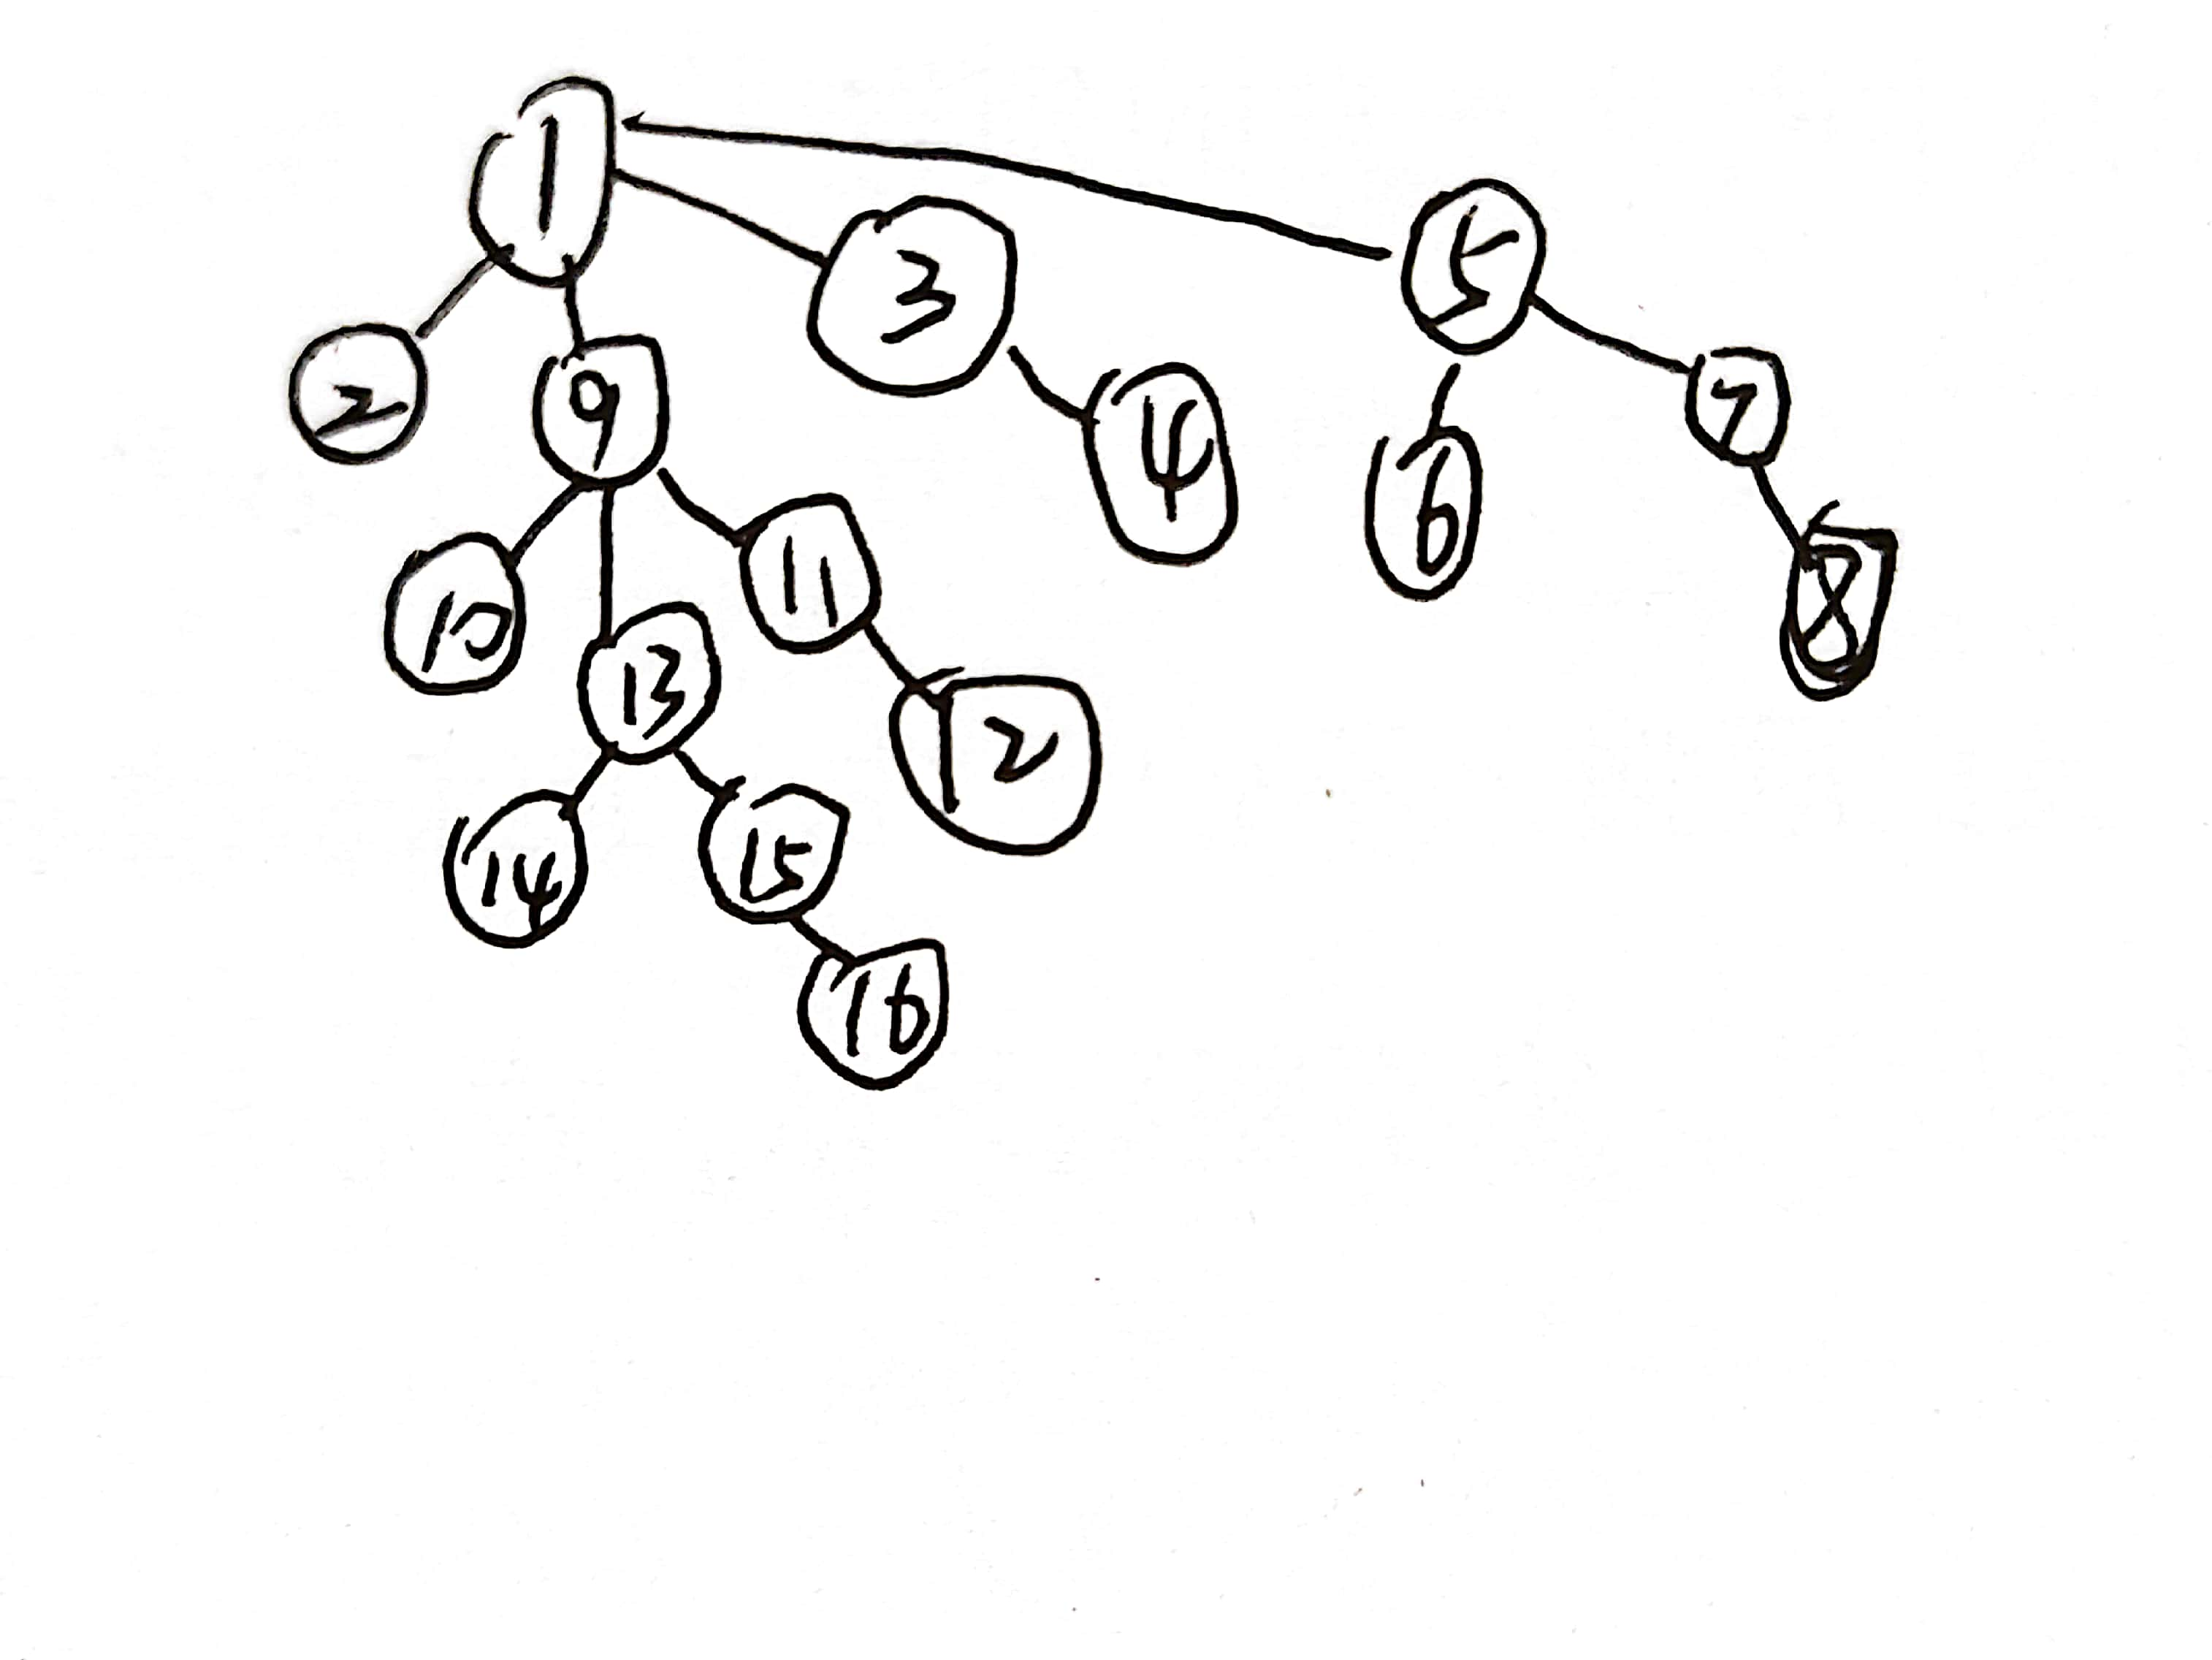
\includegraphics[width = 0.8\textwidth]{tree.jpg}
\end{solution}
%%%%%%%%%%%%%%%

%%%%%%%%%%%%%%%
\begin{problem}[TC 21.3-2]
写出使用路径压缩的FIND-SET过程的非递归版本。
\end{problem}

\begin{solution}
  \begin{algorithm}[H]
    \begin{algorithmic}[1]
      \Function{FIND-SET}{$x$}
      \State $tmp = x$
      \While{$tmp.p \neq tmp$}
      \State $tmp = tmp.p$
      \EndWhile
      \While{$x \neq tmp$}
      \State $x.p = tmp$
      \State $x = x.p$
      \EndWhile
      \State \Return tmp
      \EndFunction
    \end{algorithmic}
  \end{algorithm}
\end{solution}
%%%%%%%%%%%%%%%

%%%%%%%%%%%%%%%
\begin{problem}[TC 21.3-3]
给出一个包含$m$个MAKE-SET、UNION和FIND-SET操作的序列(其中有n个是MAKE-SET操作),当仅使用按秩合并时,需要$\Omega(m\lg n)$的时间。
\end{problem}

\begin{solution}
  \begin{algorithm}[H]
    \begin{algorithmic}[1]
      \Procedure{TC 21.3-3}{}
      \For{$i \gets 1 to n$}
      \State $MAKE-SET(x[i])$
      \EndFor
      \For{$i \gets 1 to k$}
      \For {$j \gets 1 to n' - 2^{i=1} by 2^i$}
      \State $UNION(x_i, x_{i+2^{j-1}})$
      \EndFor
      \EndFor
      \For {$i\gets 1 to m$}
      \State $FIND-SET(x_1)$
      \EndFor
      \EndProcedure
    \end{algorithmic}
  \end{algorithm}
\end{solution}
%%%%%%%%%%%%%%%
%%%%%%%%%%%%%%%%%%%%
\beginoptional

%%%%%%%%%%%%%%%
\begin{problem}[TC Problem 21-1 (Off-line minimum)]
\end{problem}

\begin{solution}
\end{solution}
%%%%%%%%%%%%%%%

%%%%%%%%%%%%%%%%%%%%
\beginot
%%%%%%%%%%%%%%%
%%%%%%%%%%%%%%%
\begin{ot}[Off-line LCA (TC Problem 21.3)]


\end{ot}

% \begin{solution}
% \end{solution}
%%%%%%%%%%%%%%%

\begin{ot}[Partition refinement]
  参考资料:\href{https://en.wikipedia.org/wiki/Partition_refinement}{https://en.wikipedia.org/wiki/Partition\_refinement}
\end{ot}

% \begin{solution}
% \end{solution}
%%%%%%%%%%%%%%%




% \vspace{0.50cm}
%%%%%%%%%%%%%%%
% \begin{ot}[]
% 
%   \noindent 参考资料:
%   \begin{itemize}
%     \item 
%   \end{itemize}
% \end{ot}

% \begin{solution}
% \end{solution}
%%%%%%%%%%%%%%%

%%%%%%%%%%%%%%%%%%%%
% 如果没有需要订正的题目,可以把这部分删掉

% \begincorrection
%%%%%%%%%%%%%%%%%%%%

%%%%%%%%%%%%%%%%%%%%
% 如果没有反馈,可以把这部分删掉
\beginfb

% 你可以写
% ~\footnote{优先推荐 \href{problemoverflow.top}{ProblemOverflow}}:
% \begin{itemize}
%   \item 对课程及教师的建议与意见
%   \item 教材中不理解的内容
%   \item 希望深入了解的内容
%   \item $\cdots$
% \end{itemize}
%%%%%%%%%%%%%%%%%%%%
% \bibliography{2-5-solving-recurrence}
% \bibliographystyle{plainnat}
%%%%%%%%%%%%%%%%%%%%
\end{document}